\documentclass[../main.tex]{subfiles}
\graphicspath{{\subfix{../images/}}}

\begin{document}

    \chapter{Sviluppo ed Automazione su Cloud}
	
    \begin{figure}[h]
		\centering
		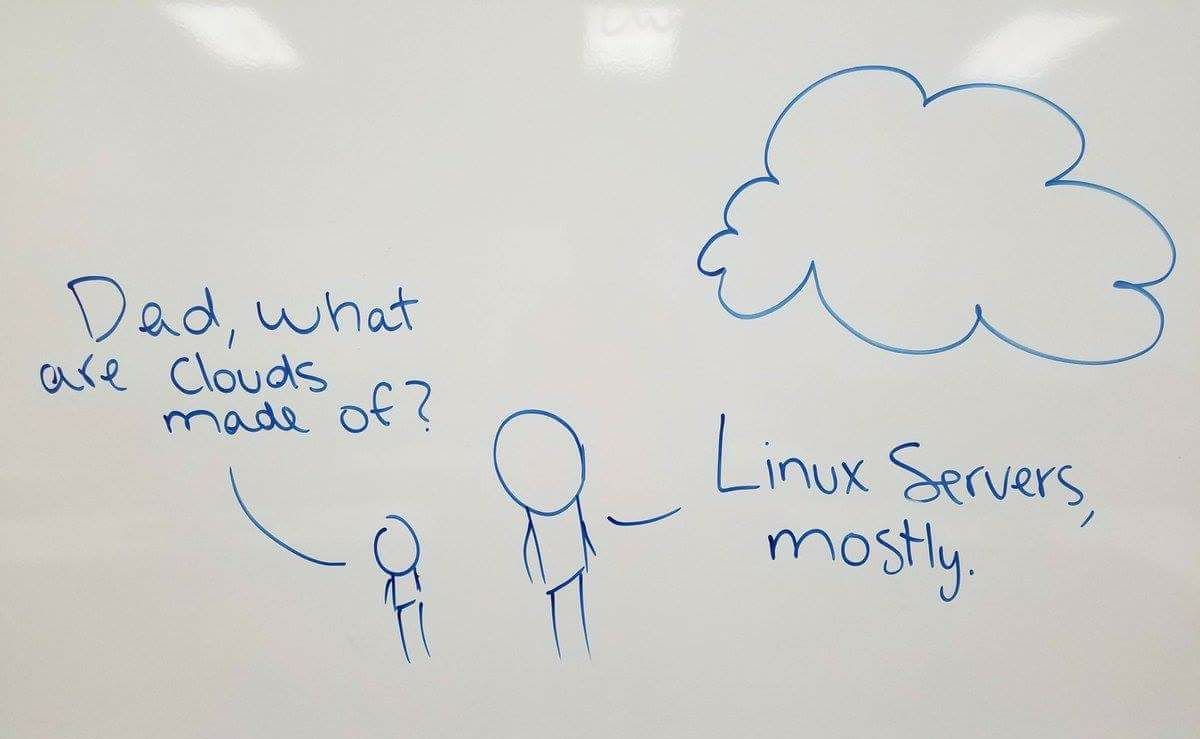
\includegraphics[width=0.6\textwidth]{cloud_meme}
    \end{figure}

        \section{Introduzione}
        
            Si sente spesso parlare in ambito informatico del concetto di \textbf{Cloud Computing}, ma il termine in se può avere diverse accezioni in base al tipo di "cloud" di cui parliamo. Il concetto generale vede il cloud come un nuovo paradigma per il quale le risorse informatiche vengono \emph{localizzate} all'esterno della rete locale e vengono sfruttate come una \textbf{entità manipolabile e configurabile}, senza limiti di utilizzo o scalabilità.
            
            In altre parole, per definire il \emph{Cloud Computing} si necessita che:
            \begin{itemize}
                \item l'utente sia in grado di ottenere risorse informatiche \emph{on-demand} senza l'interazione umana con i fornitori dei servizi;
                \item le risorse siano accessibili in modo libero da qualsiasi device o altra risorsa nella rete, che sia privata o pubblica;
                \item le risorse del fornitore siano fruibili da più utenze contemporaneamente, usando schemi multi-utente o \emph{multi-tenant}, isolamento a livello logico o di rete, ed allocabili velocemente ed elasticamente (scalabili);
                \item i sistemi si auto-gestiscano, regolando la fruizione delle risorse, sfruttando sistemi di monitoraggio automatico basati su adeguati livelli di astrazione logica e fisica. L'utilizzo deve poter essere monitorato sia dal fornitore che dal fruitore delle risorse, in tempo reale.
            \end{itemize}
    	    
    	    \paragraph{Tipologie}
    	    Seguendo la definizione di cloud del \textbf{NIST}\cite{cloud_nist}, esistono diversi modelli di erogazione dei servizi:
    	    \begin{itemize}
    	        \item \textbf{Public Cloud}: risorse disponibili mediante internet pubblico, fruibili in modo gratuito (ma limitato) oppure a consumo (generalmente orario). I sistemi public cloud permettono una scalabilità totalmente trasparente all'utilizzatore e virtualmente infinita;
    	        \item \textbf{Private Cloud}: utilizzato quasi esclusivamente da imprese, e gestita generalmente dalle stesse, ubicando le risorse \emph{on-premise} oppure in location esterne. E' concepita per andare incontro alle esigenze delle aziende che necessitano sicurezza e contenimento dei dati all'interno dell'ambiente aziendale stesso;
    	        \item \textbf{Hybrid Cloud}: unione delle prime due tipologie, generalmente nasce dalla partnership tra una azienda ed un provider di public cloud, così da poter mantenere parte delle risorse \emph{on-premise} (più sensibili) e una parte sul public cloud, così da facilitare la fruibilità da parte di interni ed esterni.
    	    \end{itemize}
    	    
    	    \begin{figure}[h]
    			\centering
    			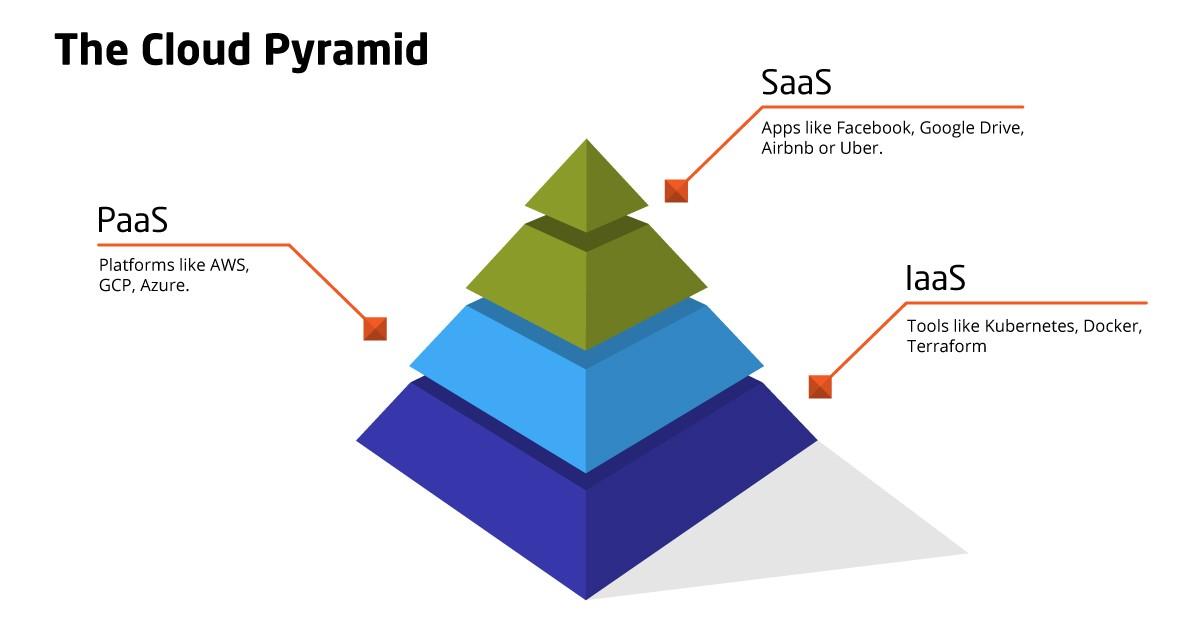
\includegraphics[width=0.8\textwidth]{cloud_pyramid}
    			\caption{La Piramide del Cloud - \textbf{Source:} Vladimir Fedak}
    			\label{fig:cloud_pyramid}
    	    \end{figure}
    	    
    	    \paragraph{Modelli di Servizio}
    	    Sempre il \textbf{NIST} definisce un modello noto come \emph{SPI}:
            \begin{itemize}
                \item \textbf{Infrastructure-as-a-Service}: mette a disposizione macchine virtuali (VM), storage virtuale ed infrastrutture di rete virtuali che i fruitori possono creare e configurare a piacere. Il provider fornisce quindi una infrastruttura \emph{bare metal} dove poi il cliente dovrà costruire il proprio pacchetto e sviluppare applicativi sul sistema operativo;
                \item \textbf{Platform-as-a-Service}: offre una versione semplificata di infrastruttura, oltre a servizi di sistema operativo, applicativi, framework di sviluppo e metodi di controllo degli stessi. Il cliente può così creare i propri applicativi unendo infrastrutture \emph{bare metal} ad applicazioni gestite dalla piattaforma;
                \item \textbf{Software-as-a-Service}: ambiente puramente applicativo, gestito dal provider, con interfaccia utente o \emph{API} sfruttabili dall'utente.
            \end{itemize}
    
            Tipica caratteristica di tutti i modelli di Cloud, è il fornire servizi secondo un \textbf{SLA} (\emph{Service Level Agreement})\cite{cloud_sla}, ovvero un contratto dove si definiscono le metriche di qualità del servizio che devono essere rispettate dal fornitore nei confronti dei propri clienti. Generalmente il \emph{SLA} si articola in definizione degli indicatori di qualità, realizzazione di un sistema di reporting, condivisione dei valori target e monitoraggio dei valori rilevati.
    
        \section{\emph{Infrastructure-as-Code}}
        
            In un ambiente \emph{Cloud}, dove le risorse sono definibili mediante \emph{API} e semplici richieste al provider dei servizi, è nata una pratica volta ad unificare lo sviluppo del codice per la definizione di intere infrastrutture in ottica \emph{DevOps}, permettendo così di sfruttare sia sviluppatori che operationals per gestire ciò che ospiterà l'applicativo sviluppato in un progetto.\\*
            
            L'\emph{Infrastructure-as-Code}\cite{cloud_iac} è quindi il processo che gestisce delle infrastrutture mediante l'utilizzo di codice \emph{machine-readable} al posto di configurazioni manuali o interfacce grafiche. Nel tempo le infrastrutture informatiche sono state oggetto di processi sempre manuali, gli addetti andavano fisicamente nel datacenter ad installare un nuovo server per poi configurarlo e renderlo fruibile a tutti.
            
            Il primo problema che si andava a creare è certamente il \textbf{costo}, mantenere molte figure in grado di gestire una infrastruttura di un certo calibro fa lievitare i costi annuali notevolmente, oltre al grado aggiunto di gestione del personale che aggiunge un altro livello di overhead sui processi. I problemi successivi riguardano la \textbf{scalabilità} e \textbf{affidabilità} delle risorse installate, che necessitavano di continue revisioni e modifiche fisiche.
            
            \begin{figure}[h]
    			\centering
    			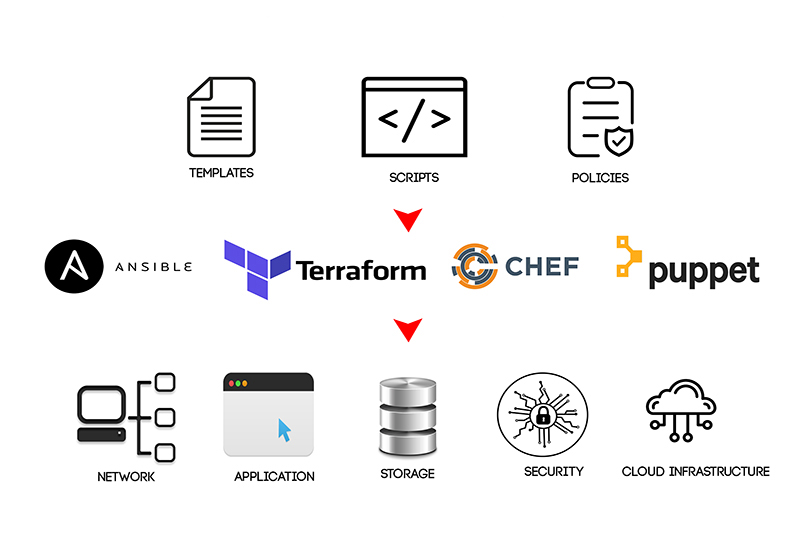
\includegraphics[width=0.7\textwidth]{cloud_iaac}
    			\caption{Infrastructure-as-Code - \textbf{Source:} HashRoot}
    			\label{fig:cloud_iaac}
    	    \end{figure}
            
            L'avvento del \emph{Cloud Computing} ha permesso di eliminare molti di questi problemi o di trovare un modo per mitigarli efficacemente, e l'\textbf{IaC} può essere definito come il "tassello mancante" a poter eliminare tutti quei processi manuali, spesso proni ad errori o a lavoro usa e getta. L'infrastruttura viene così definita a livello di codice, mediante l'uso di linguaggi diffusi o di configurazioni sempre versionabili, portando così diversi vantaggi ai processi:
            \begin{itemize}
                \item \textbf{Velocità}: creare una infrastruttura cloud diventa estremamente semplice anche per chi non ha skills puramente sistemistiche, e diventa semplice replicarla su più ambienti (dev/stg/prod);
                \item \textbf{Consistenza}: se un processo manuale può portare ad errori e risultati inconsistenti, nell'IaC il codice è l'unica \emph{"source of truth"}, che definisce tutto, dalle risorse al processo per crearle, modificarle e distruggerle;
                \item \textbf{Tracciabilità}: essendo semplice codice, può essere utilizzato un VCS per tenere traccia delle sue modifiche e nel caso effettuare dei rollback;
                \item \textbf{Efficienza}: il processo ne risente positivamente dall'uso di IaC, ad esempio per creare ambienti di testing sempre uguali e replicabili all'infinito anche da uno sviluppatore, e in fase di deployment finale sfruttare lo stesso codice per gli ambienti di produzione;
                \item \textbf{Costi}: l'utilizzo del cloud e dell'IaC permette di ridurre e tenere sott'occhio continuo i costi della propria infrastruttura, oltre a risparmiare sul personale addetto alla sua creazione e manutenzione.
            \end{itemize}
            
            L'approccio al codice può essere di tipo \textbf{imperativo} o \textbf{dichiarativo}, in base al tool scelto, dove con imperativo si intende il "come" devo modificare o creare le risorse, mentre nel dichiarativo si parte da uno stato desiderato delle cose ed il sistema deciderà le cose da fare in base allo stato attuale. Questo codice può inoltre essere integrato nei processi \emph{DevOps-oriented}, permettendo di estendere l'automazione in modo che si riesca a creare anche l'infrastruttura oltre che deployare il software creato.
            
            I principali strumenti e framework per l'\emph{Infrastructure-as-Code} sono:
            \begin{itemize}
                \item HashiCorp Terraform (multicloud)
                \item AWS CloudFormation
                \item Microsoft Azure Resource Manager
                \item Google Cloud Deployment Manager
            \end{itemize}
    
        \section{\emph{Configuration-as-Code}}
        
            Se mediante l'\emph{Infrastructure-as-Code} possiamo definire, creare e gestire le risorse infrastrutturali, una volta create queste andranno configurate e i propri applicativi installati e mantenuti. La pratica di \emph{Configuration-as-Code}\cite{cloud_cac} permette di sfruttare lo stesso concetto visto precedentemente, applicandolo ad un diverso ambito, anche se strettamente correlato se non addirittura a volte sovrapponibile con l'IaC.
            
            Questa pratica permette di eliminare ciò che veniva fatto post installazione di nuovi server fisici, ovvero \textbf{installazione, configurazione e pubblicazione degli applicativi} su di essi, o semplicemente la configurazione degli ambienti dove poi sarebbero stati installati futuri applicativi in sviluppo. Mediante la definizione di codice \emph{machine-readable} e auto-documentante, possiamo creare un sistema di configurazione unificato e sempre adatto all'ambiente in cui si trova, grazie alla possibilità di analizzare i sistemi \emph{as-is} e poi agire di conseguenza via codice.\\*
            
            I vantaggi della \emph{IaC} si riflettono quindi anche sulla \emph{CaC}, grazie all'uso di un sistema di VCS e al trattamento del codice come unica sorgente di verità, oltre che contenente lo stato desiderato dei sistemi. La CaC permette quindi di avere le seguenti feature in modo semplificato:
            \begin{itemize}
                \item Sviluppo di processi di build e deployment;
                \item Creazione di ambienti dipendenti da determinate configurazioni;
                \item Integrazione degli ambienti nei processi di Quality Assurance;
                \item Gestione di chiavi e \emph{secrets} in modo controllato.
            \end{itemize}
            
            I principali strumenti e framework per il \emph{Configuration-as-Code} sono:
            \begin{itemize}
                \item Red Hat Ansible
                \item Chef
                \item Puppet
            \end{itemize}
            
            Da notare come questi strumenti siano anche utilizzabili come \emph{Infrastructure-as-Code}, potendo fare all'effettivo entrambi i compiti in modo efficiente, ma con approccio più orientato alla configurazione piuttosto che alla creazione.
    
        \section{\emph{Containers} ed ambienti controllati}
        \label{sec:cloud_containers}
    
            Nel mondo delle infrastrutture IT, ci si è sempre preoccupati di riuscire a creare un ambiente di sviluppo o deployment più consolidato possibile, in modo da evitare mancanze di dipendenze, librerie o configurazioni necessarie al corretto funzionamento di un determinato applicativo. L'unità di misura sempre utilizzata è la \emph{"macchina"}, che può essere un server fisico, oppure un server virtuale (VM), dove poi si dovevano installare e configurare tutte le dipendenze dell'applicativo da deployare.\\*
            
            Un \textbf{container}\cite{cloud_container} è invece una unità più piccola, definibile come un ambiente software in grado di eseguire ed isolare dall'esterno l'esecuzione di uno o più processi, prendendo spunto dal container fisico utilizzato nella logistica, dove il contenuto da trasportare rimane al suo interno ma il mezzo di trasporto può cambiare frequentemente (camion, treni, navi) senza cambiamenti nel modo in cui viene gestita quell'unità.
            
            \begin{figure}[h]
    			\centering
    			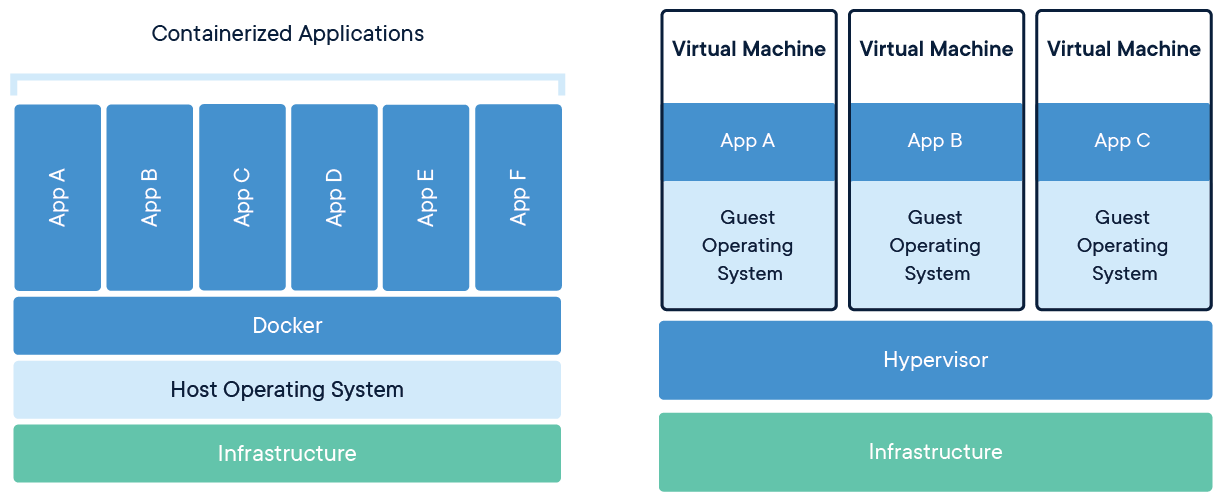
\includegraphics[width=0.8\textwidth]{cloud_containers}
    			\caption{Dalle VM ai Container - \textbf{Source:} Docker}
    			\label{fig:cloud_containers}
    	    \end{figure}
            
            Allo stesso modo un container software risulta una unità facilmente trasferibile e deployabile in molti ambienti, \emph{self-contained} ma che necessita di appoggiarsi ad un \emph{runtime} che fornisca una "base" su cui lavorare. Questo concetto non è decisamente nuovo, esistendo in modalità diverse fin dai primi anni 2000 su \textbf{FreeBSD} mediante le \emph{\textbf{jails}}, ovvero divisioni dell'OS in parti indipendenti che però condividono lo stesso \emph{kernel}. Queste implementazioni si sono poi evolute negli \emph{\textbf{LXC}} (\emph{Linux Containers}) nel 2008, la prima vera implementazione completa di un container in ambiente Linux, sopra il quale poi si sono diffusi diversi runtime di gestione quali \emph{Warden} e \emph{Docker}. Il concetto di container diventa "open" nel 2015 grazie alla nascita della \emph{\textbf{OCI}} (\emph{Open Container Initiative}), fondata da \emph{Docker}, \emph{CoreOS} e altre aziende del settore. Nel mentre anche in ambienti Windows, Microsoft implementa la possibilità di avere container nativi sui propri sistemi operativi.\\*
            
            L'utilizzo di containers in ambito Cloud permette di sviluppare applicativi \emph{agnostici} rispetto all'ambiente in cui vengono deployati, spostando così la creazione dell'ambiente corretto verso lo sviluppatore, che conosce le dipendenze necessarie al suo funzionamento. In un ambiente \emph{DevOps-oriented}, dove il team è cross-funzionale, questi container possono essere utilizzati in modo estensivo in tutte le fasi del processo, dal testing alla delivery fino al deployment finale, permettendo di facilitare notevolmente tali fasi e di evitare il cosidetto \emph{vendor lock}, ovvero la forte dipendenza da una piattaforma o ambiente per utilizzare un determinato applicativo.\\*
            
            \begin{figure}[h]
    			\centering
    			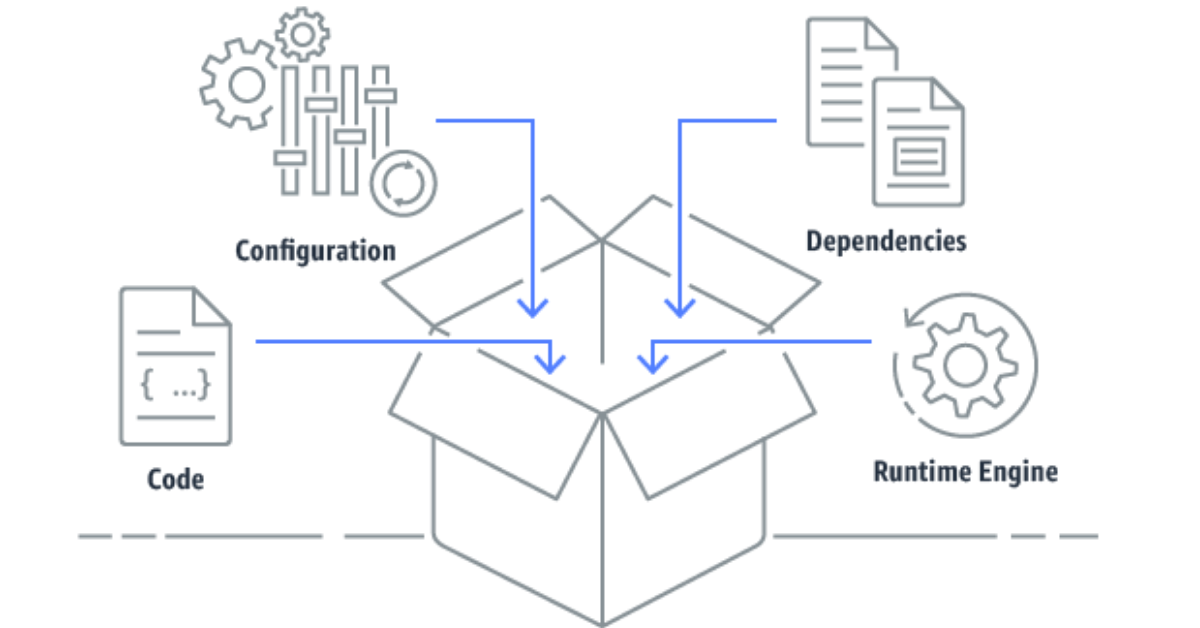
\includegraphics[width=0.7\textwidth]{cloud_container_inside}
    			\caption{Contenuto di un Container - \textbf{Source:} AWS}
    			\label{fig:cloud_container_inside}
    	    \end{figure}
            
            La stessa cosa può inoltre essere applicata agli \textbf{ambienti di sviluppo locali}; infatti sulle singole macchine degli sviluppatori si possono gestire le dipendenze del progetto sfruttando sempre dei container, che possono essere quindi creati e distrutti a piacere per fare testing e build locali, senza preoccuparsi di avere un ambiente non in linea con il resto della catena produttiva. Un esempio potrebbe essere un applicativo basato sulla \emph{Java Virtual Machine}, dove le dipendenze spesso non sono solo la macchina virtuale in se ma anche tutte le librerie accessorie; si può quindi pacchettizzare la JVM assieme al resto delle dipendenze in un singolo container, dove poi si potrà inserire l'applicativo pronto all'uso oppure sfruttarlo per creare build locali funzionanti.\\*
            
            I principali \emph{container engine}\cite{cloud_container_runtime} attualmente sul mercato sono:
            \begin{itemize}
                \item Docker RunC (basato su \emph{libcontainer})
                \item Red Hat crun (containers OCI)
            \end{itemize}

\end{document}